\documentclass[../main.tex]{subfiles}
\graphicspath{{\subfix{images/}}}

\begin{document}

\section{Results}
In the following two sections, the results of the experiments will be given. First, the changes in content 
will be shown for whenever a user is actively watching conspiracy content. Afterwards, the results for the
second experiment are set forth, wherein users are trying to escape a filter bubble after they have ended 
up in one. The results of both experiments are in part based on the predictions made by the classifier. An 
overview of the performance of the different classifiers, together with an explanation of why the 
support-vector machine was chosen to do the predictions, can be read in section \ref{ML_results}.

\subsection{The recommended content}
\subsubsection{The types of recommendations}
\begin{figure}[h]
  \textbf{Conspiracy recommendations}\par\medskip
  \centering
  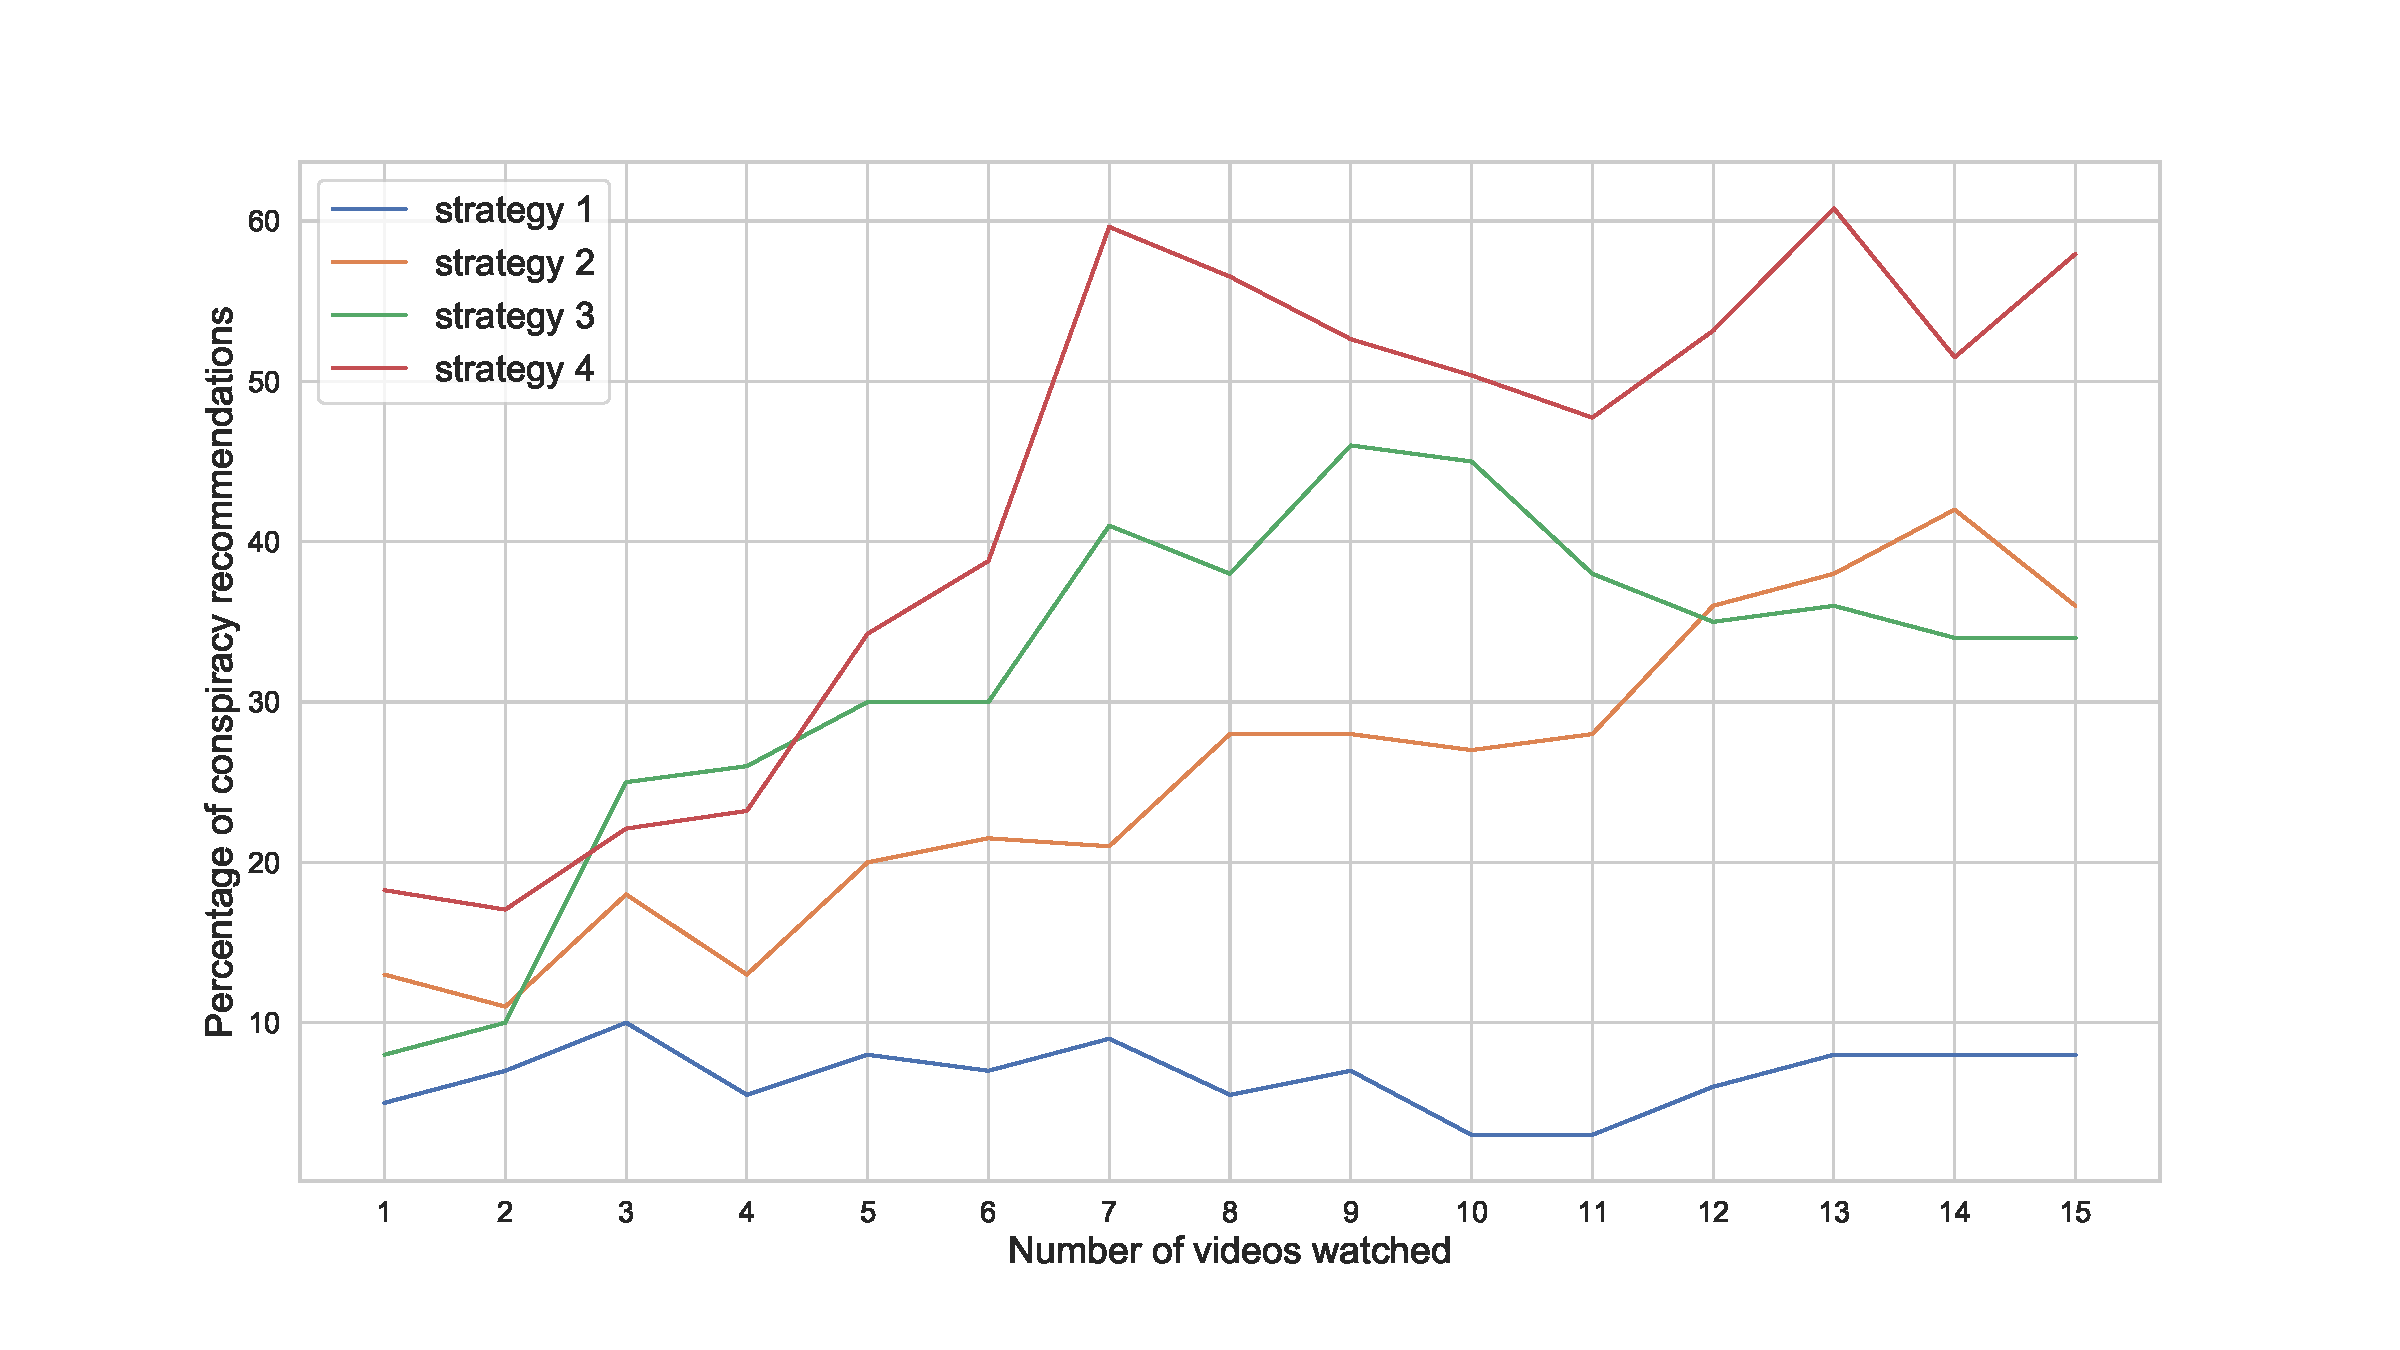
\includegraphics[keepaspectratio, width=\textwidth]{images/conspiracy_recs.pdf}
  \caption[]{The average ($N=5$) percentage of conspiracy recommendations after each number of videos watched per strategy. Each measure is based on the top twenty (20) recommendations of the five accounts for the strategy. A dashed line indicates a significant difference compared to the baseline (strategy 1) at $\alpha = 0.05$.\footnotemark}
  \label{fig:con_recs}
\end{figure}

\footnotetext{Significance for each measure was tested using multiple independent-samples t-tests. The tests compared the five percentage values after each number of videos watched per strategy to the five percentage values of the baseline (strategy 1) at that same number of videos watched. The tests were done for each strategy individually.}

All strategies, excluding the baseline, led to an increased number of conspiracy recommendations on the 
user's homepage. For all strategies, this increase was significant, meaning filter bubbles were indeed being 
created. However, the strategies all behaved differently, as can be seen in figure \ref{fig:con_recs}. 

Strategy 2 (random conspiracy videos) took the longest out of all the strategies to get into a filter bubble. 
Only after having watched six videos did the difference between it and the baseline become significant. After 
having increased significantly, the percentage of conspiracy videos being recommended to the users of strategy 2
kept steadily growing, eventually plateauing at 42\%. 

Strategy 3 (top conspiracy recommendation next to the watched video) got into a bubble the quickest. After 
watching only three videos did the difference compared to baseline become significant. However, following this 
head start, the increase came to a halt rather quickly. After reaching its peak of 46\% at nine videos watched, 
the percentage of conspiracy recommendations started to decline again, eventually settling around 35\%. Though 
most values are slightly higher, strategy 3's course mimics that of strategy 2 until the decline. 

Strategy 4 (top conspiracy recommendation on the YouTube homepage) took slightly longer to get into a filter 
bubble than strategy 3. However, considering that these strategies are identical up until video five and the 
difference between the two strategies was insignificant ($p > 0.05$), this dissimilarity is negligible. As soon 
as homepage recommendations started getting watched, the percentage of conspiracy recommendations increased 
drastically, reaching a peak of 60.8\%. Similarly to strategy 3, once the number of conspiracy recommendations 
reached a peak, it was followed by a decrease. 

To better understand how the different strategies affected the recommendations provided by the algorithm, a 
directed network of each strategy was created and analyzed. For each strategy, the networks is constructed as 
follows: the set of nodes consists of all videos watched by the five accounts of the strategy, plus, for every 
watched video $V$ the top twenty homepage recommendations that were present after watching $V$. An edge between 
two nodes $V1$ and $V2$ indicates that for at least one bot, $V2$ was recommended directly after watching $V1$. 
The different networks are displayed in figure \ref{fig:rec_net}. It can be seen that strategies
1 and 2 have barely any cross-class edges (strategy 1 has two in total, strategy 2 has zero), while 
strategies 3 and 4 have a lot of connections between the two separate classes. This stronger connection also 
becomes apparent when looking the networks' betweenness centrality and clustering coefficient (table 
\ref{tab:net_metrics}). 

\begin{table}[b]
\centering
\begin{tabular}{lrr}
\toprule
{} &  Betweenness centrality &  Clustering coefficient \\
\midrule
Strategy 1 &            1.597418e-07 &                0.001592 \\
Strategy 2 &            0.000000e+00 &                0.000000 \\
Strategy 3 &            2.198488e-06 &                0.009512 \\
Strategy 4 &            1.136934e-04 &                0.039018 \\
\bottomrule
\end{tabular}
\caption{\label{tab:net_metrics} The average betweenness centrality and clustering coefficient of each strategy's network. A node having a higher betweenness centrality indicates that it is present on more shortest paths between other nodes, meaning it is located more centrally within the network. A higher clustering coefficient indicates the network as a whole is more clustered, meaning more ties between triplets are present.}
\end{table}

\begin{table}
\centering
\begin{tabular}{lrrrr}
\toprule
{} &    $P(C \mid R)$  & $P(R \mid C)$ &    $P(C \mid C)$ &  $P(R \mid R)$ \\
\midrule
Strategy 1 &  0.065493 &       NaN &       NaN &  0.934507 \\
Strategy 2 &       NaN &  0.750000 &  0.250000 &       NaN \\
Strategy 3 &  0.185714 &  0.663043 &  0.336957 &  0.814286 \\
Strategy 4 &  0.105263 &  0.560673 &  0.439327 &  0.894737 \\
\bottomrule
\end{tabular}
\caption[]{\label{tab:cond-probs} Conditional probabilities of cross- and within-class edges for each network. Values indicate the probability of an edge going to a class, given it starts in another (in the form: $P(end \mid start)$).\footnotemark}
\end{table}

\footnotetext{In other words, the values represent the conditional, class-dependent out-degrees of the nodes. The probabilities therefore can be interpreted as the likelihood of a node belonging to a certain class having an outgoing edge to a node of the same or opposite class.}

When looking at the conditional probabilities of cross- and within-class edges per network (table 
\ref{tab:cond-probs}), it can be seen that regardless of the strategy, regular videos are highly likely to 
recommend more regular videos. However, the more personalized the strategy, the higher the probability of 
conspiracy videos recommending more conspiracy videos. This supports the creation of filter bubbles, as 
users are more likely to be recommended content similar to that which they already watched. This is also 
shown in the probability of cross-class edges for the strategies: the more personalized the strategy, the 
lower the probability of cross-class edges being present. This, too, can cause filter bubbles, as users are 
less likely to be recommended content that is different from that which they have already watched. 

When solely looking at the conspiracy recommendations of each strategy, it once more becomes clear that the 
recommendations of strategies 3 and 4 are connected more strongly than those of strategies 1 and 2 (appendix 
\ref{appendix:networks}). However, these networks are somewhat deceiving, as an edge not being present does not 
necessarily indicate there is no link between the two nodes; it could also simply be that the recommendations 
coming from that node were not checked (i.e., the recommendation was not chosen to be watched, hence its 
outgoing recommendations could not be stored). Yet, even with these missing edges, the clustering coefficient 
and betweenness centrality of strategies 3 and 4 end up being higher than those of strategies 1 and 2, as can be
seen in table \ref{tab:sub-net_metrics}. 

\begin{table}[h]
\centering
\begin{tabular}{lrr}
\toprule
{} &  Betweenness centrality &  Clustering coefficient \\
\midrule
Strategy 1 &                0.000000 &                0.000000 \\
Strategy 2 &                0.000000 &                0.000000 \\
Strategy 3 &                0.000012 &                0.016064 \\
Strategy 4 &                0.000747 &                0.058816 \\
\bottomrule
\end{tabular}
\caption{\label{tab:sub-net_metrics} The average betweenness centrality and clustering coefficient of each strategy's sub-network consisting of only conspiracy recommendations.}
\end{table}

\begin{figure}
  \textbf{The recommendation network of each strategy}\par\medskip
  \centering
  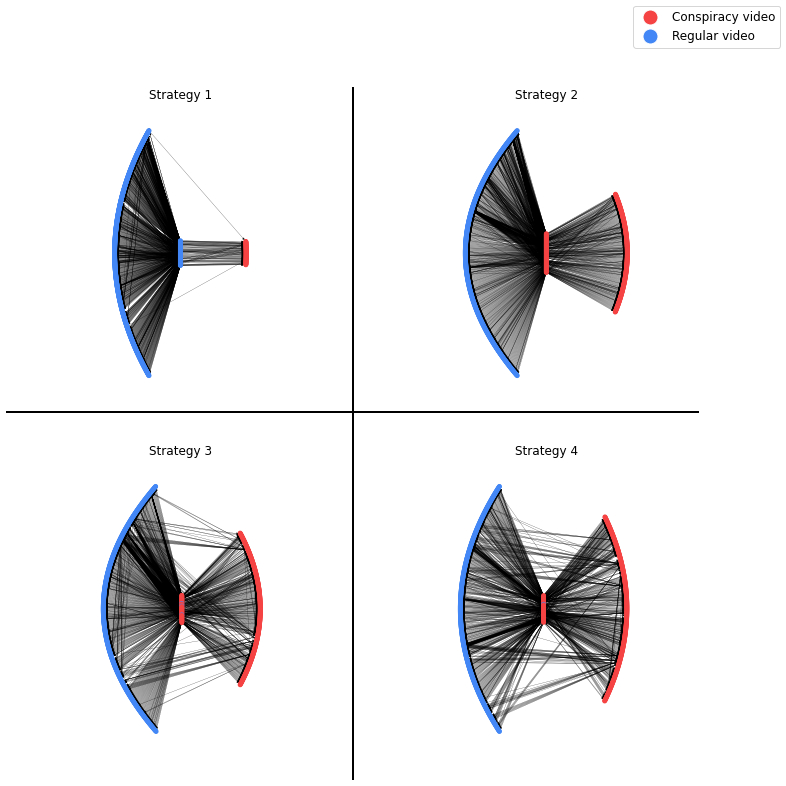
\includegraphics[keepaspectratio, width=\textwidth]{images/recommendation networks.png}
  \caption{The networks of recommendations of each strategy. Nodes on the left indicate regular (non-conspiracy) recommendations, nodes in the middle indicate the 75 videos that were watched by the bots (fifteen videos, times five bots), and nodes on the right are conspiracy recommendations. A node can be present in both the middle and either the left/right group, as some of the recommendations were watched by the bots, therefore also counting as watched videos. An edge not being present does not always indicate a link between videos was not present, as not all recommendations were watched (and thus not all links could be checked).}
  \label{fig:rec_net}
\end{figure}

\newpage

\subsubsection{Characteristics of the recommended content}
\begin{figure}
  \textbf{Cosine similarity of recommendations}\par\medskip
  \centering
  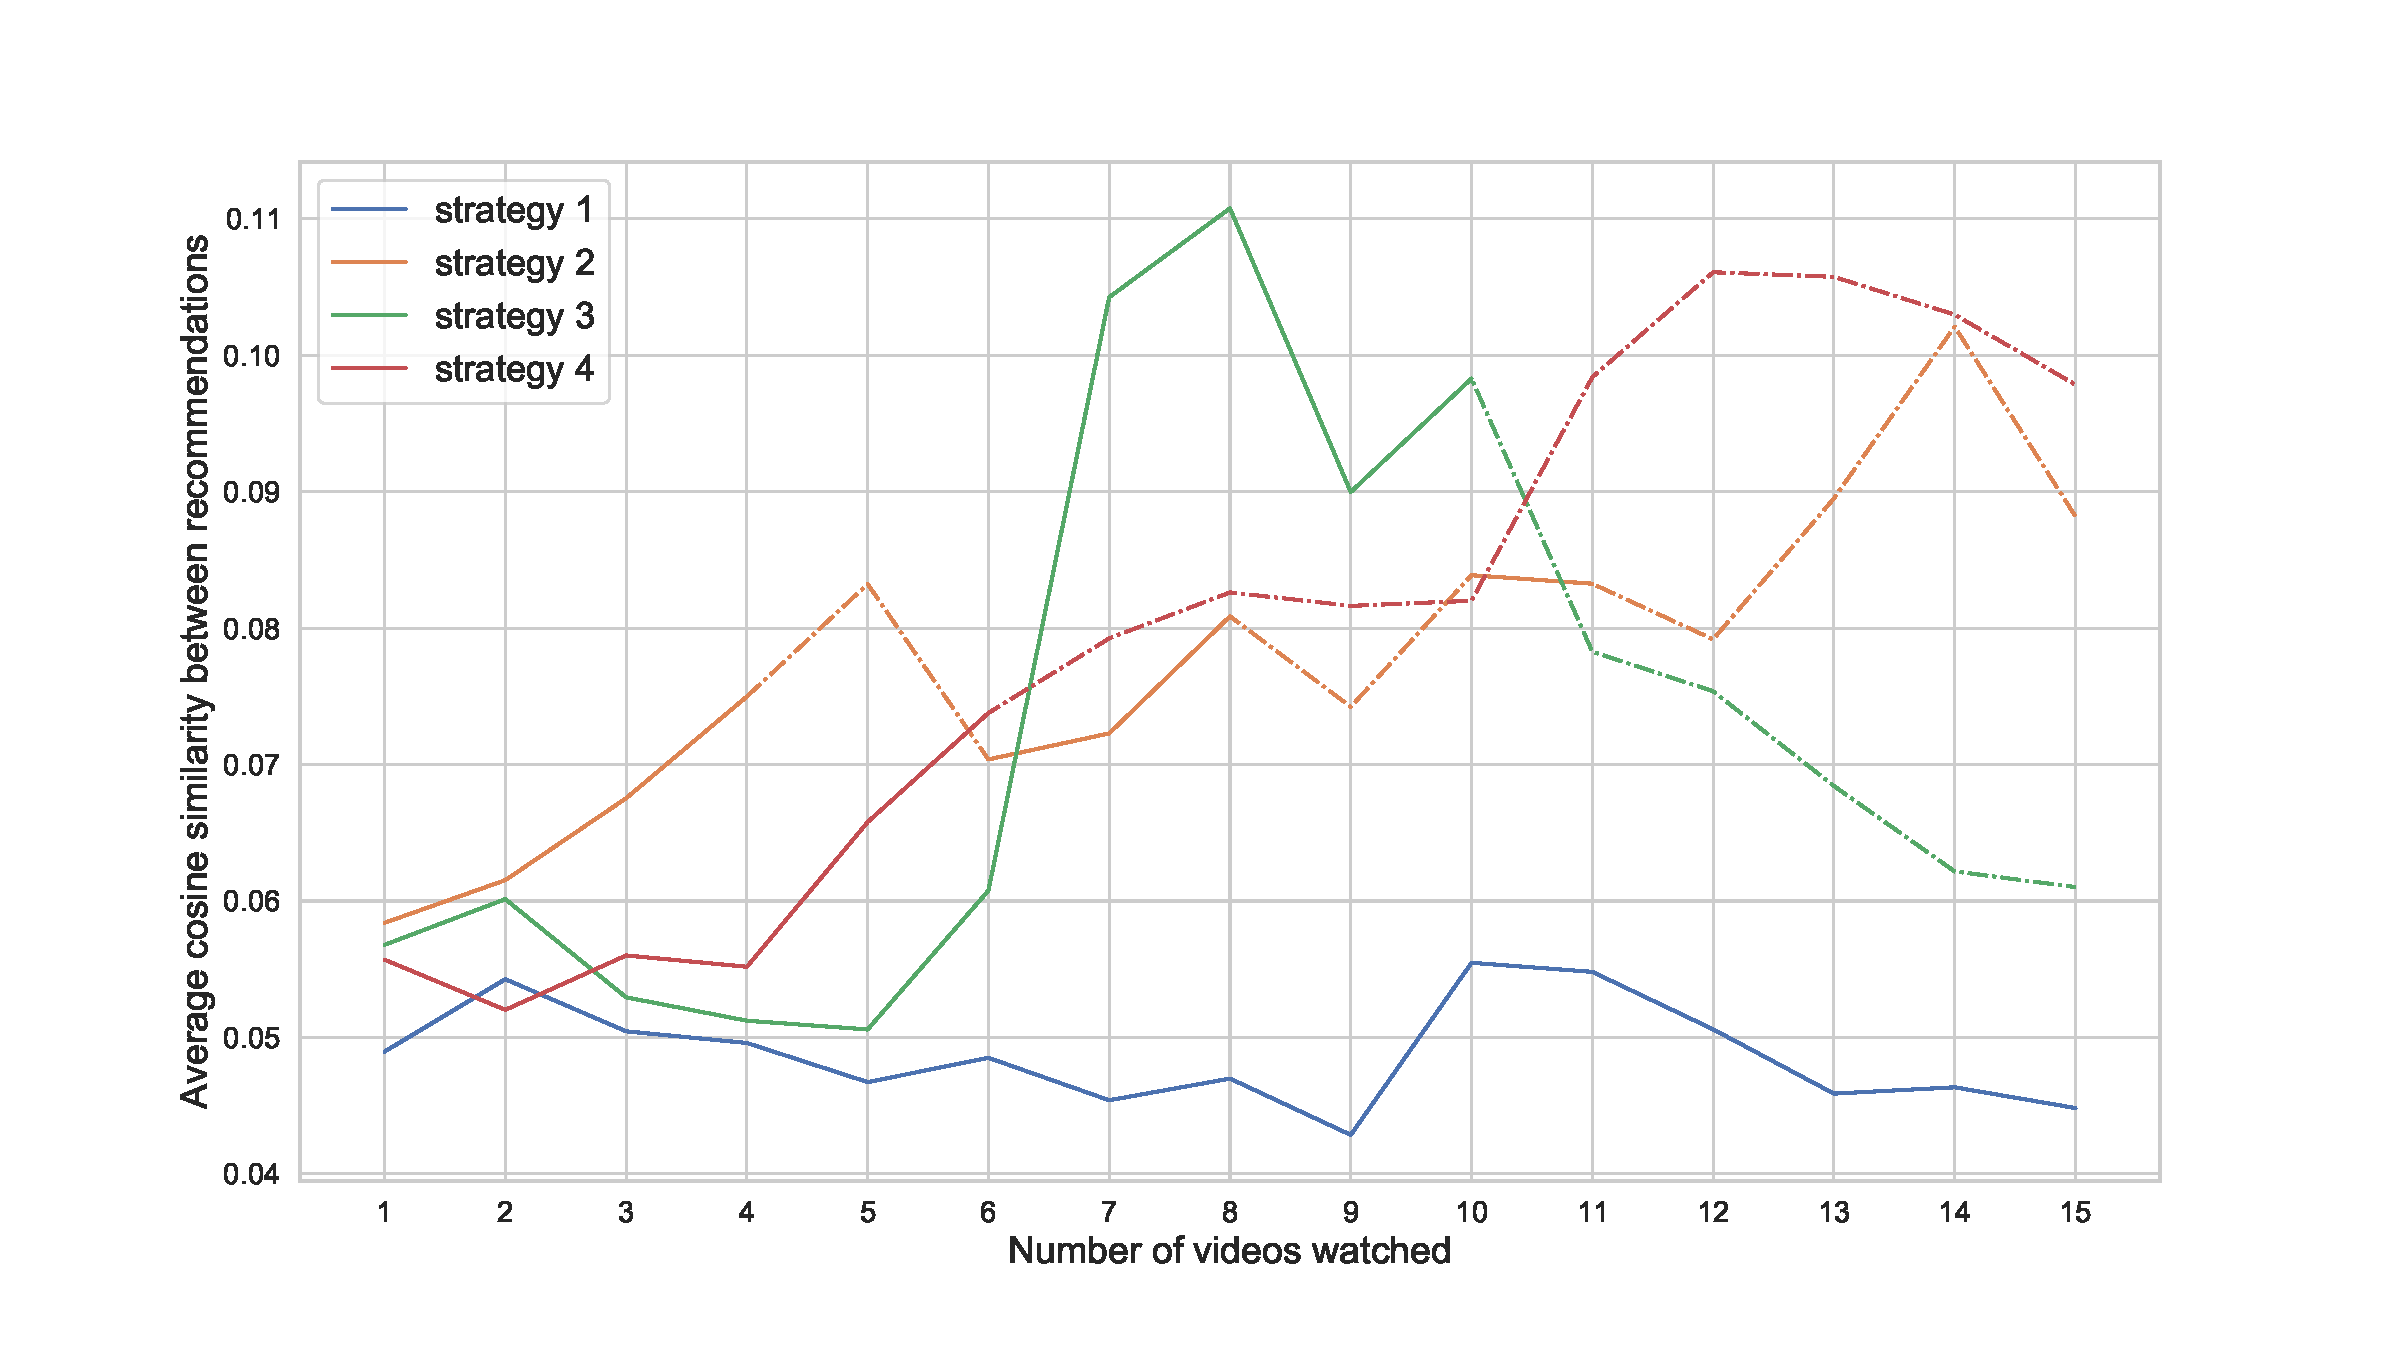
\includegraphics[keepaspectratio, width=\textwidth]{images/All sim.pdf}
  \caption{The average cosine similarity of the homepage recommendations per strategy after each number of videos watched (based on the TF-IDF representations of the recommendations). Each measure consists of the first twenty recommendations of the five users for each strategy. A dashed line indicates a significant difference compared to the baseline (strategy 1) at $\alpha = 0.05$.}
  \label{fig:similarities}

\centering
\begin{minipage}[b]{0.45\linewidth}
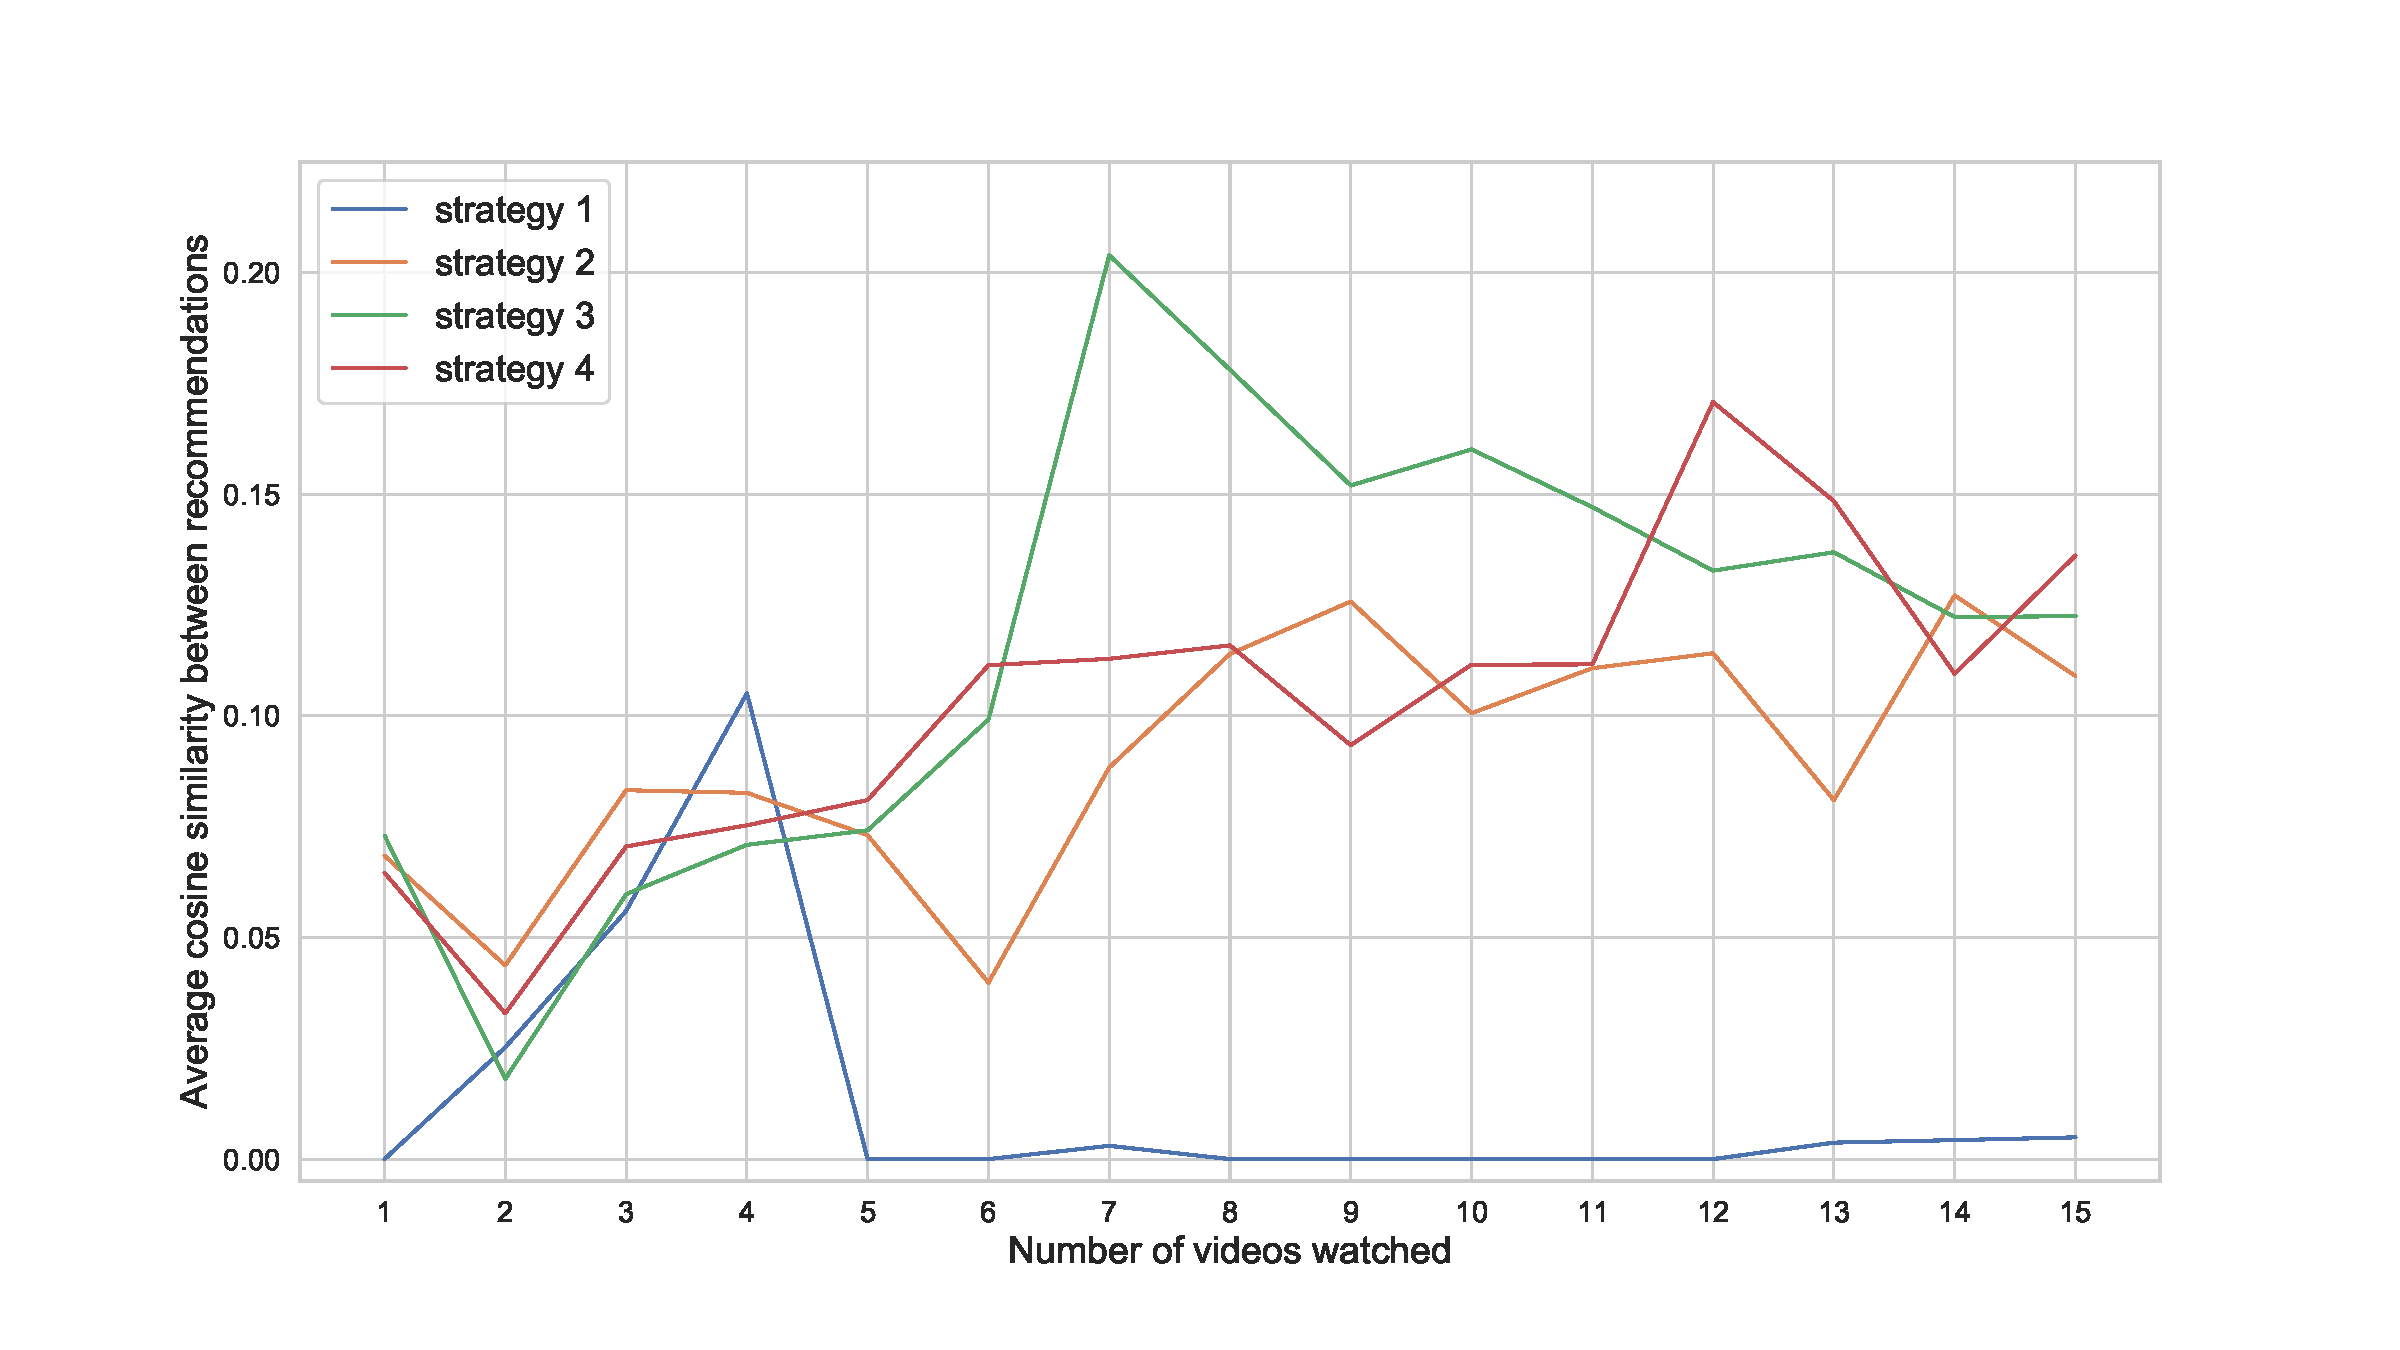
\includegraphics[width=\textwidth]{images/Con sim.pdf}
\caption{Cosine similarity of conspiracy videos}
\label{fig:con_sim}
\end{minipage}
\quad
\begin{minipage}[b]{0.45\linewidth}
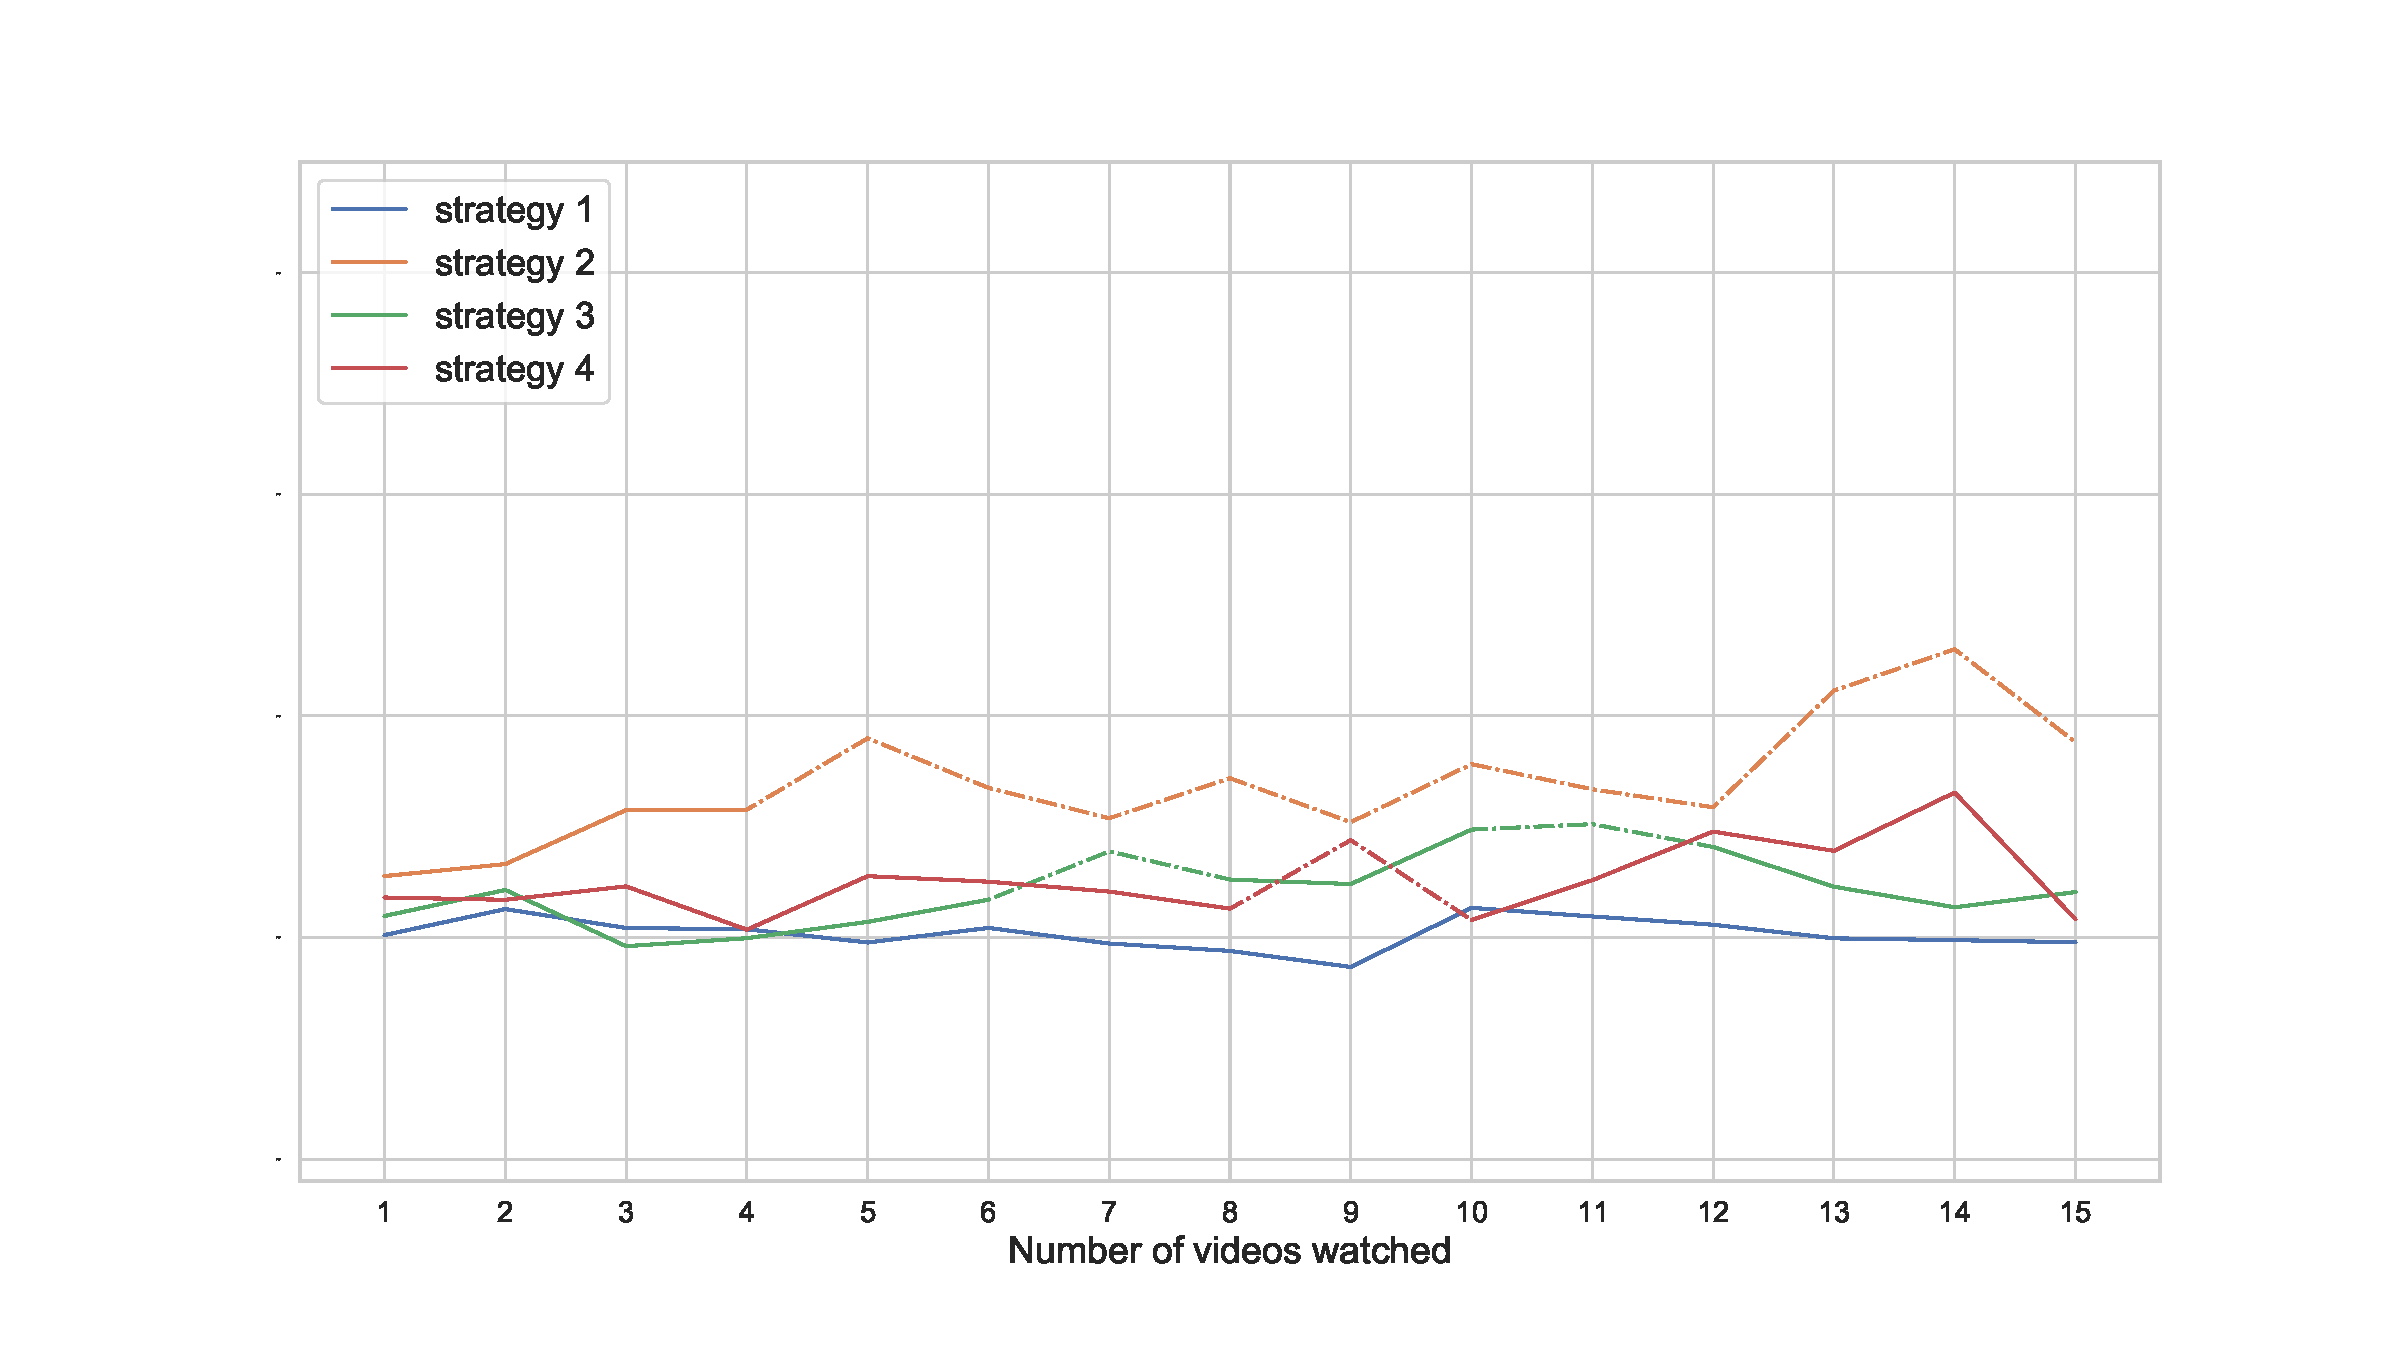
\includegraphics[width=\textwidth]{images/Reg sim.pdf}
\caption{Cosine similarity of regular videos}
\label{fig:reg_sim}
\end{minipage}
\end{figure}


\paragraph{Recommendation similarity}
Every strategy, excluding the baseline, eventually led to a decreased diversity of the recommended content. The 
similarity of the recommended content increased relatively slowly, however. When compared to the speed with 
which the recommendations started to prefer conspiracy content, the number of videos that needed to be watched 
until the average cosine similarity between recommendations became significantly higher than that of the 
baseline is quite high (figure \ref{fig:similarities}). 

Surprisingly, strategy 2 actually was the first strategy for which the difference in content-similarity 
became significant; considering the bots watched random conspiracy videos, it is surprising that the 
recommendations became similar at all. However, this only lasted for two videos, after which the difference 
became insignificant again until video nine. After having watched all fifteen videos, strategy 2 actually had 
more similar recommendations than strategy 3, which is remarkable, considering this strategy watched random 
(thus, seemingly unrelated) conspiracy videos. 

Strategy 3 took the longest for the difference compared to baseline to become significant. While its 
similarity skyrocketed after video six, this high value was caused by a single outlier, causing it not 
to be significant. Eventually, the other values caught up to the outlier to some degree, causing the result 
to become significant after all. Still, even then is the similarity lower than that of strategy 2. 

Strategy 4 took slightly longer than strategy 2 to show a significant difference. However, this significance 
never disappeared afterwards. Strategy 4's similarity increased in two separate bursts of quick growth, 
both followed by a slowdown. After fifteen videos, strategy 4's average similarity barely outperformed 
that of strategy 2, although this difference is insignificant ($p > 0.05$).

\paragraph{View count}
The average popularity of recommended videos dropped quickly for all strategies, including the baseline. For 
all strategies, the average view count of recommendations started at more than ten million. This number then 
rapidly decreased, already dropping into the single millions or hundreds of thousands after five videos
watched. Thus, YouTube starts by recommending very popular content, as that is most likely to cater to the 
largest audience. However, after the user has watched a few videos, thereby giving the algorithm a better
idea of their interests, the recommendations become more personalized and therefore less generic. 

\paragraph{Video duration}
There seemed to be no trend in the average duration of the recommended videos for any of the strategies. For 
each strategy, the average length of the recommended videos stayed between three and ten minutes, spiking up 
or down seemingly at random. Detailed graphs of the average view count and duration of recommendations can be
found in appendix \ref{appendix:views}.

\subsection{Leaving the filter bubble}

\begin{figure}[t]
  \textbf{Conspiracy recommendations when leaving the filter bubble}\par\medskip
  \centering
  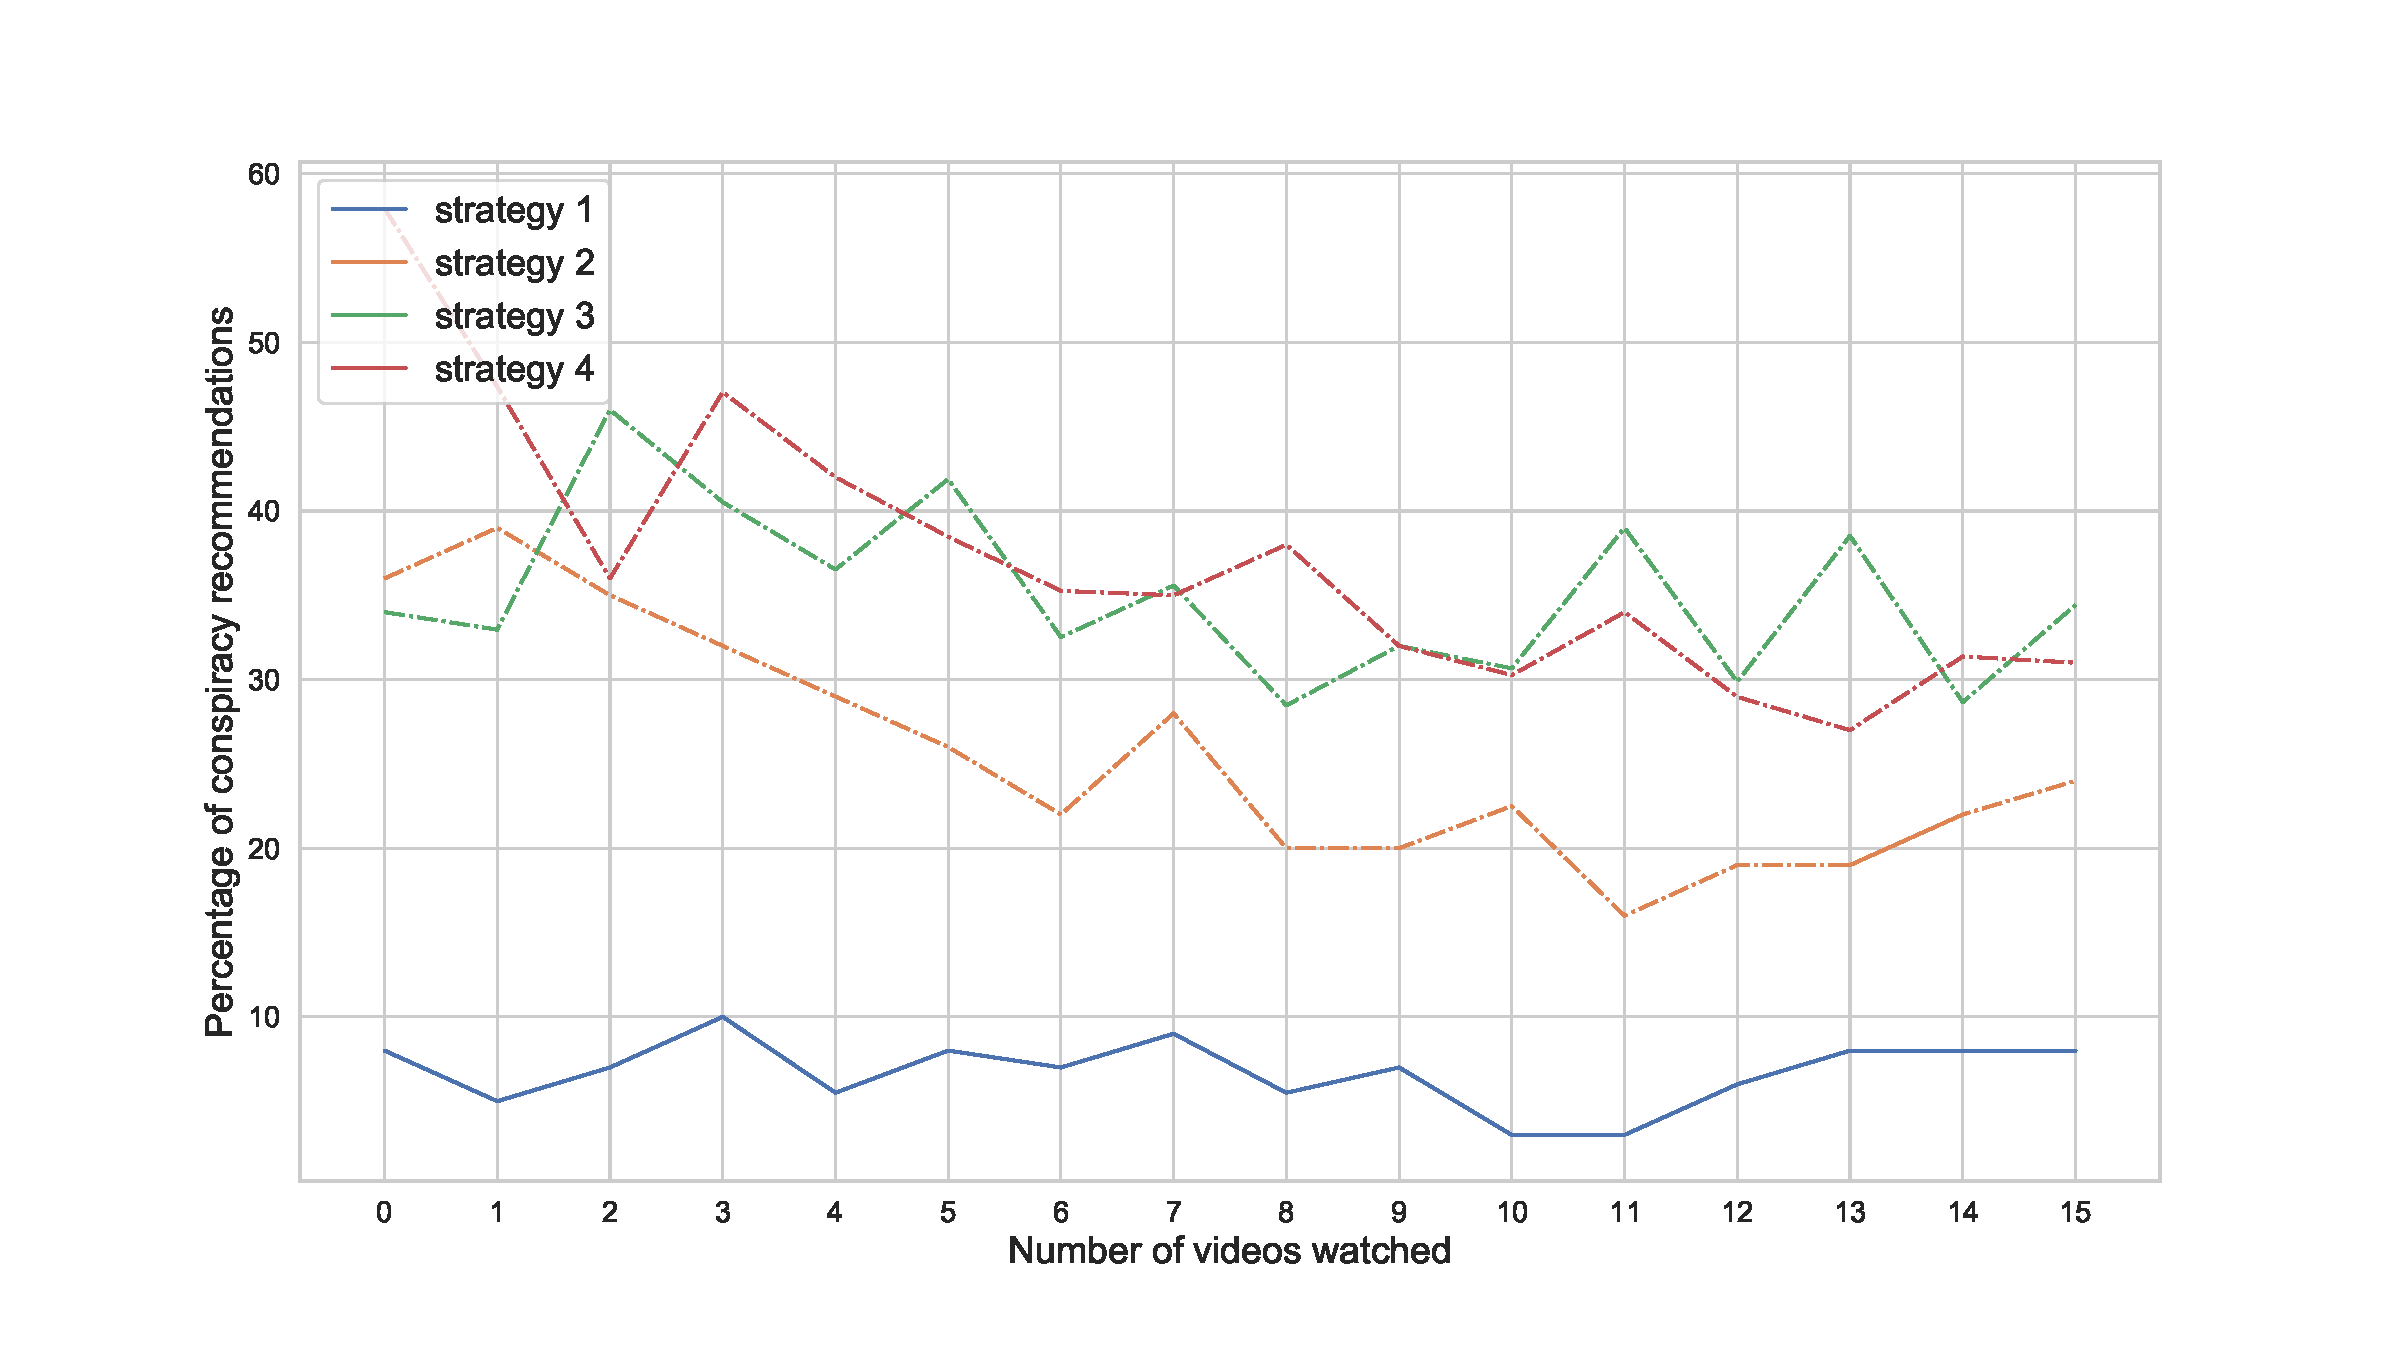
\includegraphics[keepaspectratio, width=\textwidth]{images/conspiracy_recs_2.pdf}
  \caption{The percentage of conspiracy recommendations after each number of videos watched per strategy while trying to escape a filter bubble. Each measure is based on the top twenty recommendations of the five accounts for the strategy. A dashed line indicates a significant difference compared to the baseline (strategy 1) at $\alpha = 0.05$.}
  \label{fig:con_recs_2}
\end{figure}

While it took only a handful of videos before a user's recommendations started preferring conspiracy content, 
undoing this preference required far more videos to be watched. While the algorithm quickly adjusted to the 
new type of content being watched, it did not stop recommending conspiracy content, even after the users had
watched fifteen non-conspiracy videos (figure \ref{fig:con_recs_2}). 

For all strategies, the percentage of conspiracy recommendations rapidly decreased from its initial value. 
However, the number of conspiracy recommendations soon leveled-out for all three strategies at a value still 
significantly higher than that of the baseline. In other words, while the algorithm is quick to reflect a change
in users' watching behaviour, it does not 'forget' what has been watched in the past for quite some time. 

Strategy 2 and 3 decreased by approximately the same amount, although strategy 3 constantly stayed at a
higher percentage, as that strategy's initial percentage was higher than that of strategy 2. Strategy 4 dropped
quite a bit more than the other two strategies; it ended up with practically the same values as strategy 3, even
though its initial value was over 20\% higher (57.9\% as opposed to 34\%). 

Yet, for all three strategies did the number of conspiracy recommendations not return to baseline, even after 
having watched all fifteen videos. Considering only three to six videos had to be watched before the users ended
up in a filter bubble, it is quite concerning that getting out of that bubble takes several times more videos. 
Someone can end up in a filter bubble before they even realize it, but once they are in one, it will be 
difficult for them to get out. 

\subsection{Machine learning} \label{ML_results}

\begin{figure}
  \textbf{Classifier performance}\par\medskip
  \centering
  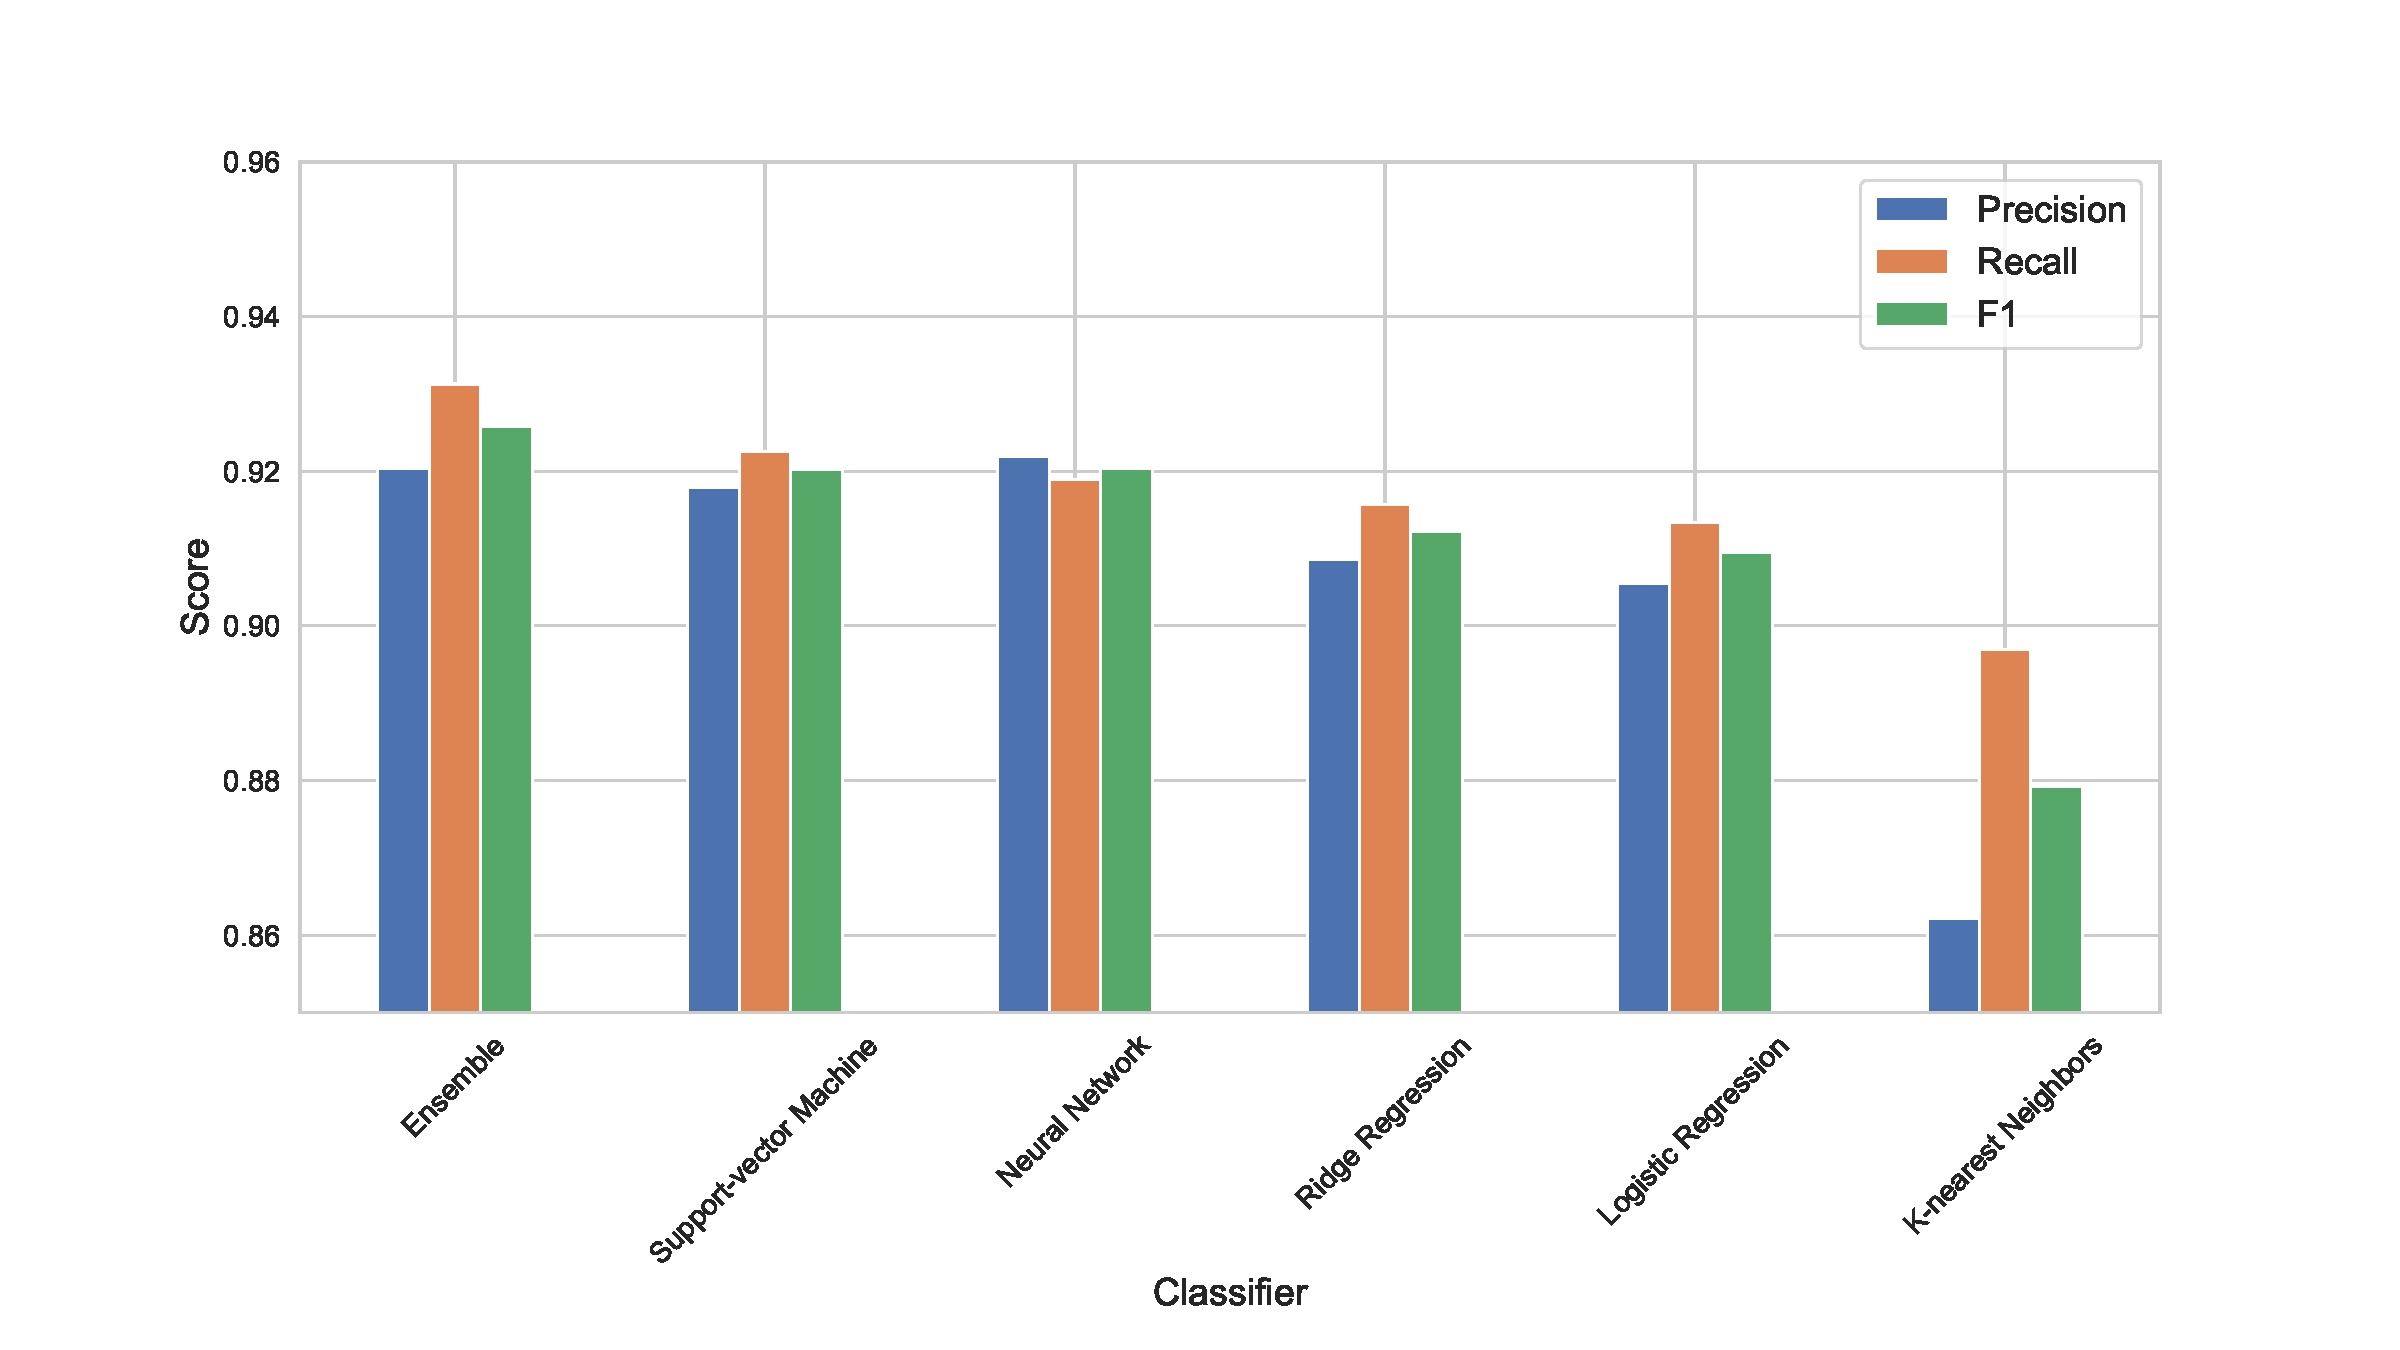
\includegraphics[keepaspectratio, width=\textwidth]{images/classifier_results.pdf}
  \caption{Metrics for each classifier with optimized hyperparameters}
  \label{fig:ML_scores}
\end{figure}

The hyperparameter tuning led to impressive scores for all classifiers. When making predictions for the
test set, the best-performing classifier is the support-vector machine making use of the Radial Basis
Function (RBF) kernel and a penalty parameter (C-value) of 10. The SVM is tied for F1-score with the neural 
network using the identity activation function, with 10 hidden layers of 10 neurons. Ridge regression with a 
sparse-cg solver and penalty (alpha) value of 0.1 takes the third place, very closely followed by logistic 
regression with an L2 penalty, a penalty (C) value of 20 and a newton-cg solver. The worst-performing 
classifier is also the simplest of the bunch: the k-nearest neighbors classifier (K=1). Although its 
performance is still formidable, it does substantially worse than the others. An overview of all metrics for 
each classifier can be seen in figure \ref{fig:ML_scores}. The ten best-performing configurations for each
classifier can be found in appendix \ref{appendix:Hyperparameters}.

Noteworthy is the fact that the optimal ensemble actually outperforms the support-vector machine by a
slight margin. This ensemble, consisting of the SVM, the neural network, and surprisingly, the k-nearest
neighbor classifiers, gets slightly higher scores than the runner-up across the board. The ensemble had
a 16-way tie for best-performing parameters, all of which contained at least the SVM, neural network,
and k-NN classifiers. 

Though the ensemble outperforms the other classifiers, it has a significant drawback: its training time
is significantly larger than that of the individual classifiers. Support-vector machines are infamous
for their slowness when there is a lot of training data, and neural networks can require a lot of
training time whenever the number of neurons gets large \citep{burges1997improving,
kamarthi1999accelerating}. Requiring both algorithms to run will therefore require a lot of additional
training time. Considering the marginal performance increase, the cost outweighs the benefit. As a
result, when taking everything into account, the support-vector machine is the best classifier for
labeling conspiracy videos on YouTube.

Additionally, for predicting the likelihood of recommendations being conspiracy videos in real-time, the 
best-performing classifier is the neural network. The predicted likelihood was used to find the most-likely 
conspiracy recommendation after each video watched, which was done for strategy 3 and 4. Here, the neural 
network is preferred over the support-vector machine, as neural networks are better optimized for providing 
probabilities of samples belonging to a certain class \citep{specht1990probabilistic}.
\end{document}